\newpage
\section{The Program}
\subsection{Database schema}
\hspace{0.7cm}The database below is our database system. It describes in detail the relationship between the components in the system and the characteristics of each element in the system.

\vspace{2cm}
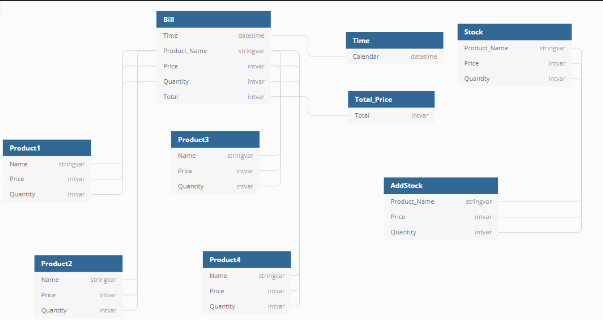
\includegraphics{images/database.png}

\newpage
\vspace{6cm}
\subsubsection{Relationship between tables}
\begin{itemize}
 \item Bill: it is shown on the user structure
  \item Stock: it is shown on the user structure
  \item Time: it connects to the Bill table
  \item AddStock: it's only linked to the Stock table
  \item Product: it links to Bill and Stock tables
  
\end{itemize}

\vspace{0.5cm}
\subsubsection{Tables’ functions}
\begin{itemize}
  \item Bill: it includes: Time, Product Name, Price, Quantity, Total Bill of custumers.
  \item Stock: it includes all information of new product.
  \item Time: it provides information in the form of "dates" for the Bill and Stock tables.
  \item AddStock: it is used to enter information of new products as they are entered into the store.
  \item Product: It includes information of that product such as: price, quantity, name.
\end{itemize}

\newpage
\subsection{Python modules, classes and packages}
\hspace{0.7cm}Here are the Modules, classes and packages used in our program:

\vspace{1cm}
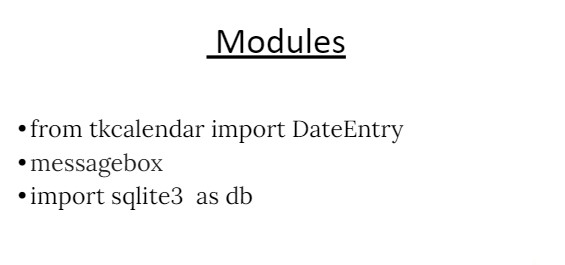
\includegraphics{images/modules.jpg}



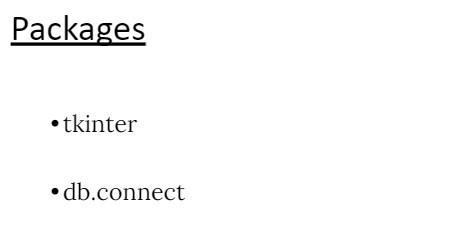
\includegraphics{images/packages.jpg}



\begin{enumerate}
  \item \textbf{"db.connection"} package: contains everything related to the database
    \begin{itemize}
        \item \textbf{"funiturestoremanagentsystem.SQL"} file: the database of the store in SQL file
        \item \textbf{"FunitureStoreManagentSystem.py"}: a Python module that deals with the database. It has 3 classes: 
            \begin{itemize}
                \item \textbf{class Bill} With the bill class, it contruct the component and the properties of each component like:productname, price, date, quantity;
                
                \item \textbf{class Storage} with Stock class, it helps the user to import a new product into the storeage. Also it helps users to know what products are in storage and their data.;
                
                \item \textbf{class Connect: } connects the database to the interface. By:
                
                connectObj =db.connect("FurnitureStoreManagement.db")
                
                cur = connectObj.cursor()
            \end{itemize}
    \end{itemize}
  \item \textbf{"tkinter"} package:it helps us to get the user interface as above.
  \item \textbf{"tkcalendar"}: a Python module that provides information on transaction time as well as order entry on the user interface. 
  \item \textbf{"messagebox"}: This is a type of dialog used to display messages to the user and sometimes even to make selection requests to the user.
  
  \item \textbf{"main.py"}: another Python module that is able to run the program
\end{enumerate}